% report.tex - Frontpage for the report (place in Report/)
\documentclass[a4paper,12pt]{article}
\usepackage[utf8]{inputenc}
\usepackage[T1]{fontenc}
\usepackage{graphicx}
\usepackage{eso-pic}
\usepackage[HTML]{xcolor}
\usepackage{tikz}
\usepackage{geometry}
\usepackage{parskip}
\usepackage{setspace}
\usepackage{caption}
\usepackage{subcaption}
\usepackage{float}
\usepackage{gensymb}
\usepackage{ulem}
\usepackage{amsmath}
\usepackage{amsfonts}
\usepackage{microtype}
\usepackage{tabularx}
\usepackage{longtable}
\usepackage{booktabs}
\usepackage{hyperref}
\usepackage{makecell}
\usepackage[
backend=biber,
style=apa,
sorting=ynt
]{biblatex}
\renewcommand{\bibfont}{\small}
\addbibresource{bibliography/bibliography.bib}

\geometry{margin=2.5cm}

\AddToShipoutPictureBG{
  \definecolor{sidebar}{HTML}{008571}
  \begin{tikzpicture}[remember picture,overlay]
    \fill[sidebar]
    (current page.north west)
    rectangle
    ([xshift=1.2cm]current page.south west);
  \end{tikzpicture}
}

\begin{document}
\begin{titlepage}
    \thispagestyle{empty}
    \centering
    \vspace*{2cm}

    
\includegraphics[width=0.6\textwidth]{logos/nmbu_logo_tekst.jpeg}

    {\Huge\bfseries TEL200 - Introduction to Robotics}\\[0.5cm]
    {\Large\itshape Group 5}\\[1.5cm]

    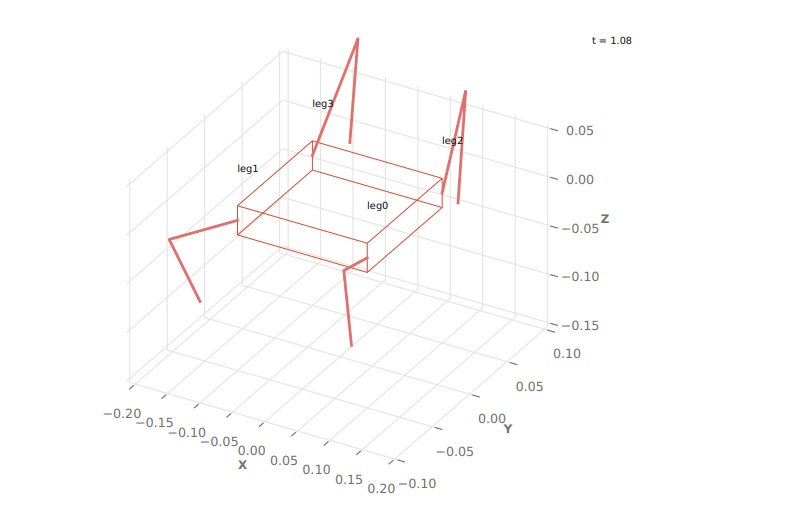
\includegraphics[width=.7\textwidth]{images/WalkingRobot.jpg}

    {\Large\itshape Walking Robot Project}\\[1.5cm]

    \rule{0.6\textwidth}{1pt}\\[0.8cm]

    {\Large\bfseries Authors}\\[0.3cm]
    {\large Andreas Brustad \\ Johannes Standal \\ Håkon Bekken}\\[1cm]

    \vfill

    \small Norwegian University of Life Sciences
\end{titlepage}

\AddToShipoutPictureBG{%
  \AtPageUpperLeft{%
    \raisebox{-2.3cm}{%
      \hspace{1.14\textwidth}%
      
\includegraphics[width=2cm]{logos/nmbu_logo.png}
    }%
  }%
}

\tableofcontents

\newpage


\section{Abstract}


% \includegraphics[...]{images/...}


\section{Introduction}


% \includegraphics[...]{images/...}


\section{Method}


% \includegraphics[...]{images/...}

%\begin{table}[H]
%  \centering
%  \caption{}
%  \begin{tabular}{c|c|c|c}
%    \toprule
%    & \textbf{X=0} & \textbf{X=1} & \textbf{X=2} \\
%    \midrule
%    \textbf{Y=0} & & & \\
%    \textbf{Y=1} & & & \\
%    \textbf{Y=2} & & & \\
%    \bottomrule
%  \end{tabular}
%\end{table}

% \includegraphics[...]{images/...}


\section{Results}


% \includegraphics[...]{images/...}


\section{Discussion}


\section{Conclusions}


\section{Bibliography}
\printbibliography

\end{document}